% !TEX TS-program = lualatex
% LuaLaTeX + luatexja 推奨。図は TikZ を使用。
\documentclass[12pt]{ltjsarticle}

% 日本語（LuaTeX-ja）と数式・図
\usepackage{luatexja}
\usepackage{amsmath,amssymb,mathtools,amsthm}
\usepackage{bm}
\usepackage{tikz}
\usetikzlibrary{arrows.meta,positioning,calc}
\usepackage[a4paper,margin=28mm]{geometry}

\title{線形代数1 第5回\; グラフと行列\;― 数学的解説と Lean 形式化の対応}
\author{（氏名をここに記入） \\ CODEX (OpenAI) — TeX 自動生成 \\ CODEX (OpenAI) — Lean ファイル生成}
\date{\today}

% 記法
\DeclareMathOperator{\diag}{diag}
\newcommand{\1}{\mathbf{1}}
\newcommand{\R}{\mathbb{R}}
\newcommand{\A}{\mathsf{A}}
\newcommand{\D}{\mathsf{D}}
\newcommand{\Lapl}{\mathsf{L}}
\newcommand{\J}{\mathsf{J}}

\begin{document}
\maketitle

\paragraph{要旨}
本稿は「線形代数1」第5回（グラフと行列）の要点を、ニコラ・ブルバキの\textit{構造の精神}（集合と写像による定式化）に沿って簡潔に解説し、同内容を Lean 4 + mathlib で形式化したファイル\texttt{src/MyProjects/LinearAlgebra/A1/zenla1\_session05.lean}との対応を示す。図は TikZ により挿入し、LuaLaTeX でのコンパイルを想定する。

\section{ブルバキ的な構造化の見取り図}
グラフは集合 $V$（頂点）と二項関係 $E\subseteq V\times V$ の組とみなせる。有限集合 $V=\{0,\dots,n-1\}$ に同型をとると、$\A\in\R^{n\times n}$ を
\[
  \A_{ij} = \begin{cases}
    1 & ((i,j)\in E)\\
    0 & \text{otherwise}
  \end{cases}
\]
と定めることで、構造（$V,E$）が\textit{行列}として表現される。写像（グラフ準同型）$f:V\to V'$ は、適切な条件の下で行列の変換（例えば添字の置換やブロック構造の保存）に対応する。これにより集合・写像の図式が線形代数的計算（行列演算）へと射影される。

\section{基本定義と記法}
頂点数 $n$ の実行列 $\A\in\R^{n\times n}$ を\textbf{隣接行列}とする。各頂点の\textbf{次数}は行和
\[
  \deg(i) := \sum_{j=0}^{n-1} \A_{ij} \in \R
\]
で与えられ、\textbf{次数行列}は $\D := \diag(\deg(0),\dots,\deg(n-1))$。\textbf{ラプラシアン行列}は
\[
  \Lapl := \D - \A.
\]
無向グラフは $\A$ が対称（$\A^{\mathsf{T}}=\A$）で特徴づけられる。完全グラフ $K_n$ の全1行列を $\J\in\R^{n\times n}$ と書くと、$K_n$ のラプラシアンは
\[
  \Lapl(K_n) = n\,I - \J
\]
である。

\section{具体例と図}
以下では $P_4$（パス）、$C_4$（サイクル）、$K_3$、$K_4$ を用いる。

\begin{figure}[h]
  \centering
  \begin{tikzpicture}[scale=1.0, every node/.style={circle,draw,inner sep=1pt}]
    % P4: 0-1-2-3
    \node (p0) at (0,0) {\small 0};
    \node (p1) at (1.8,0) {\small 1};
    \node (p2) at (3.6,0) {\small 2};
    \node (p3) at (5.4,0) {\small 3};
    \draw[-{Stealth[length=2mm]}] (p0) -- (p1);
    \draw[-{Stealth[length=2mm]}] (p1) -- (p0);
    \draw[-{Stealth[length=2mm]}] (p1) -- (p2);
    \draw[-{Stealth[length=2mm]}] (p2) -- (p1);
    \draw[-{Stealth[length=2mm]}] (p2) -- (p3);
    \draw[-{Stealth[length=2mm]}] (p3) -- (p2);
    \node[draw=none] at (2.7,-0.9) {$P_4$};

    % C4: square 0-1-2-3-0
    \begin{scope}[xshift=8.2cm]
      \node (c0) at (0,0) {\small 0};
      \node (c1) at (1.5,0) {\small 1};
      \node (c2) at (1.5,1.5) {\small 2};
      \node (c3) at (0,1.5) {\small 3};
      \foreach \u/\v in {c0/c1,c1/c2,c2/c3,c3/c0}{
        \draw[-{Stealth[length=2mm]}] (\u) -- (\v);
        \draw[-{Stealth[length=2mm]}] (\v) -- (\u);
      }
      \node[draw=none] at (0.75,-0.9) {$C_4$};
    \end{scope}
  \end{tikzpicture}
  \caption{パス $P_4$ とサイクル $C_4$（有向に描画しているが $\A$ は対称）}
\end{figure}

\begin{figure}[h]
  \centering
  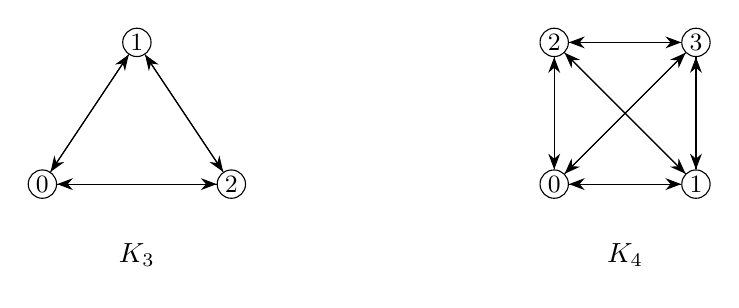
\begin{tikzpicture}[scale=1.0, every node/.style={circle,draw,inner sep=1pt}]
    % K3
    \node (k30) at (0,0) {\small 0};
    \node (k31) at (1.2,1.8) {\small 1};
    \node (k32) at (2.4,0) {\small 2};
    \foreach \u/\v in {k30/k31,k31/k32,k32/k30}{
      \draw[-{Stealth[length=2mm]}] (\u) -- (\v);
      \draw[-{Stealth[length=2mm]}] (\v) -- (\u);
    }
    \node[draw=none] at (1.2,-0.9) {$K_3$};

    % K4
    \begin{scope}[xshift=6.5cm]
      \node (k40) at (0,0) {\small 0};
      \node (k41) at (1.8,0) {\small 1};
      \node (k42) at (0,1.8) {\small 2};
      \node (k43) at (1.8,1.8) {\small 3};
      \foreach \u/\v in {k40/k41,k40/k42,k40/k43,k41/k42,k41/k43,k42/k43}{
        \draw[-{Stealth[length=2mm]}] (\u) -- (\v);
        \draw[-{Stealth[length=2mm]}] (\v) -- (\u);
      }
      \node[draw=none] at (0.9,-0.9) {$K_4$};
    \end{scope}
  \end{tikzpicture}
  \caption{完全グラフ $K_3$ と $K_4$}
\end{figure}

\section{演習（Q1–Q5）の要点}
\paragraph{Q1（$P_4$ の次数）} 端点 $0,3$ は次数 $1$、中間 $1,2$ は次数 $2$。行和で確認できる。

\paragraph{Q2（$C_4$ の無向性）} 隣接行列が対称、すなわち $\A^{\mathsf{T}}=\A$。

\paragraph{Q3（歩数と $\A^2$）} $(\A^2)_{ij}=\sum_k \A_{ik}\A_{kj}$ は長さ2の歩数。$P_4$ では $(i,j)=(0,2)$ に対し $k=1$ のみ寄与し $1$。

\paragraph{Q4（$K_3$ のラプラシアン）} $\deg(i)=2$、対角 $\A_{ii}=0$、非対角 $\A_{ij}=1$ より
\[
  \Lapl(K_3)=\begin{bmatrix}2&-1&-1\\-1&2&-1\\-1&-1&2\end{bmatrix}.
\]

\paragraph{Q5（行和は常に 0）} 任意の $i$ で
\[
  \sum_j \Lapl_{ij} = \sum_j (\D_{ij}-\A_{ij})
  = \underbrace{\sum_j \D_{ij}}_{=\deg(i)} - \underbrace{\sum_j \A_{ij}}_{=\deg(i)} = 0.
\]

\section{チャレンジ：$K_4$ の全1ベクトルは固有値 0}
全1ベクトル $\1\in\R^4$ に対し、$\Lapl(K_4)=\D-\A$ の各行和が $3-3=0$ なので $\Lapl(K_4)\,\1=\bm{0}$。一般に $K_n$ では $\Lapl=nI-\J$、$\J\,\1=n\,\1$ より $\Lapl\,\1=\bm{0}$、また $\1^{\perp}$ 上で固有値 $n$（重複度 $n-1$）。

\section{Lean 形式化との対応}
本講の Lean ファイルでは、頂点集合を \verb|Fin n| とし、\verb|Matrix (Fin n) (Fin n) \R| を隣接行列とする。
\\[-1ex]
\begin{itemize}
  \item 次数：\verb|degree A i := ∑ j, A i j|
  \item 次数行列：\verb|degreeMatrix A := diagonal (fun i => degree A i)|
  \item ラプラシアン：\verb|laplacian A := degreeMatrix A - A|
  \item 具体例：\verb|pathGraph|, \verb|cycleGraph|, \verb|K3|, \verb|K4|
  \item 全1ベクトル：\verb|allOnes n : Fin n → ℝ|
\end{itemize}
証明は \verb|simp| と有限和の恒等式（\verb|Fin.sum_univ_*|）で機械的に実行できる。

\section*{謝辞と再現性}
本 PDF と Lean ファイルの執筆・整形は CODEX (OpenAI) による自動生成支援を受けた。再現には LuaLaTeX（\verb|lualatex|）で本ファイルをコンパイルし、Lean 側は \verb|lake exe cache get; lake build| を用いる。

\end{document}

